\begin{figure}[bt!]
    \begin{center}
      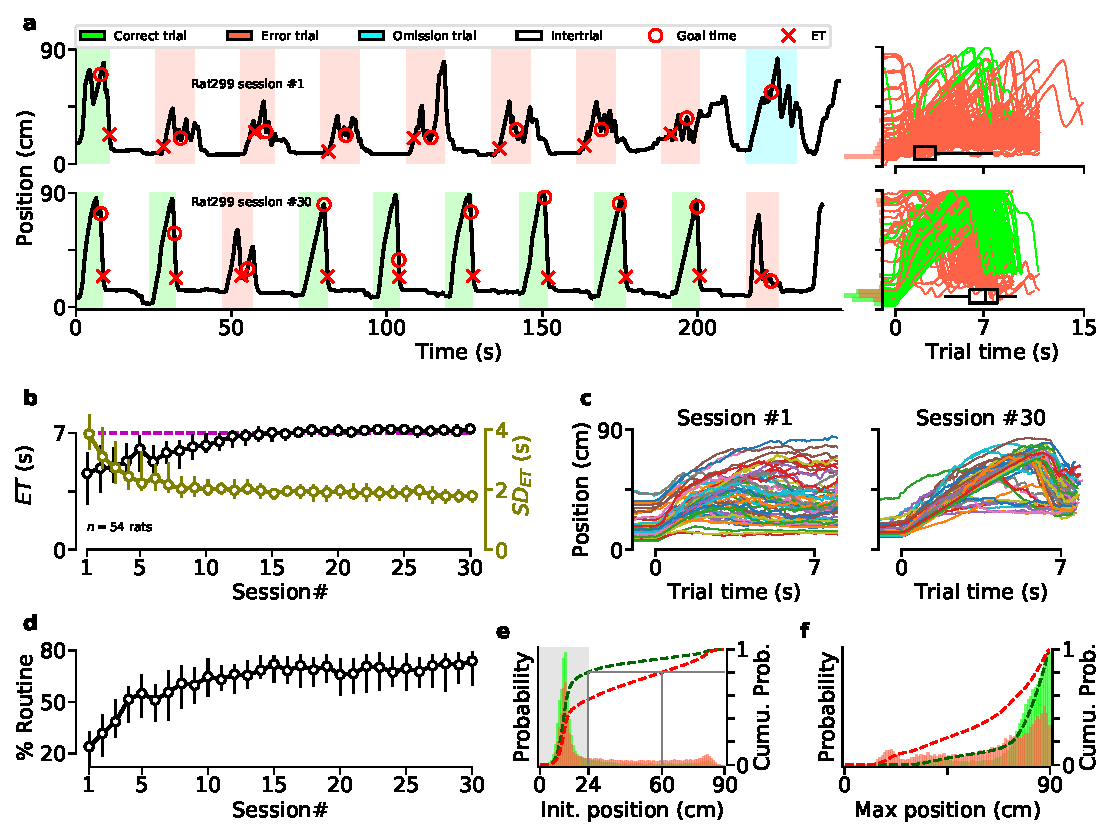
\includegraphics[width=.8\linewidth]{ch-time/figures/CtrlTrd.pdf}
      \caption[Control Condition]
      {\textbf{Most animals developed a unique stereotyped motor sequence.}
      \textbf{a)}
      \textit{Left}: illustration of an animal's trajectory on the treadmill during 9 consecutive trials of the 1st (\textit{top}) and 30th (\textit{bottom}) training sessions.
      On the y-axis, 0~and 90~indicate the treadmill's front (reward port) and rear wall, respectively.
      \textit{Right}: trajectories for all trials during the 1st (\textit{top}) and 30th (\textit{bottom}) sessions (same animal as in left panels).
      Distributions of initial positions for correct (green) and error (red) trials are shown on the y-axis.
      Black horizontal boxplots depict entrance time range (center line, median; box, 25th and 75th percentiles; whiskers, 5th and 95th percentiles).
      \textbf{b)}
      Median entrance time ($ET$) in the reward area for the first 30 daily training sessions.
      Circles indicate group median and error bars, the median range (25th and 75th percentiles) across animals for $ET$ and on the right y-axis,$SD$ of $ET$~($SD_{ET}$) values.
      The dashed magenta line shows the goal time (7~s).
      \textbf{c)}
      Median trajectory of all the trials for the 1st (\textit{left}) and 30th (\textit{right}) training sessions.
      Each line represents a single animal~($n=54$).
      \textbf{d)}
      Session-by-session percentage of trials during which animals performed the stereotyped front-back-front routine (see \nameref{ch:methods:methods}).
      Circles indicate group median and error bars, the median range across animals (25th and 75th percentiles).
      \textbf{e)}
      Probability distribution function~(PDF) of the position of the animals at the beginning of each correct (green) and error (red) trial, from sessions \#20 to \#30.
      Dashed lines represent cumulative distribution functions (right y-axis).
      The gray area indicates that in trained animals,~80\% of correct trials began with the animal located near the front of the treadmill.
      \textbf{f)}
      PDF of the maximum position along the treadmill reached by animals before crossing the beam~($=ET$).
      Only trials in which animals were initially located in the front of the treadmill (gray area in panel~e) were included.
    }
    \label{fig:time:CtrlTrd}
    \end{center}
  \end{figure}